\usetikzlibrary{arrows.meta}

\begin{frame}{register renaming: missing pieces}
    \begin{itemize}
    \item what about ``hidden'' inputs like \texttt{\%rsp}, condition codes?
    \item one solution: translate to intructions with additional register parameters
        \begin{itemize}
        \item making \%rsp explicit parameter
        \item turning hidden condition codes into operands!
        \end{itemize}
    \item bonus: can also translate complex instructions to simpler ones
    \end{itemize}
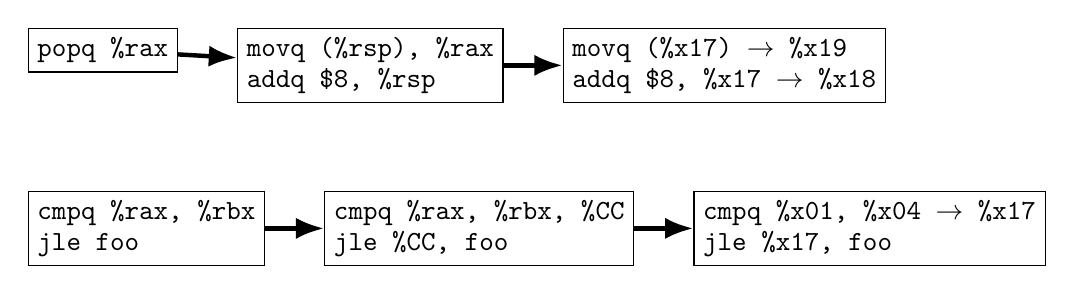
\begin{tikzpicture}
\node[draw,font=\fontsize{10}{11}\tt\selectfont] (push start) {
    popq \%rax
};
\node[draw,font=\fontsize{10}{11}\tt\selectfont,anchor=north west,align=left] (push second) at ([xshift=.75cm]push start.north east) {
        movq (\%rsp), \%rax \\ addq \$8, \%rsp
};
\node[draw,font=\fontsize{10}{11}\tt\selectfont,anchor=north west,align=left] (push third) at ([xshift=.75cm]push second.north east) {
        movq (\%x17) $\rightarrow$ \%x19 \\ addq \$8, \%x17 $\rightarrow$ \%x18 
    };
\draw[ultra thick,-Latex] (push start) -- (push second);
\draw[ultra thick,-Latex] (push second) -- (push third);
\node[draw,font=\fontsize{10}{11}\tt\selectfont,anchor=north west,align=left] (cmpjmp start) at ([yshift=-1.5cm]push start.south west) {
    cmpq \%rax, \%rbx \\
    jle foo
};
\node[draw,font=\fontsize{10}{11}\tt\selectfont,anchor=north west,align=left] (cmpjmp second) at ([xshift=.75cm]cmpjmp start.north east) {
    cmpq \%rax, \%rbx, \%CC \\
    jle \%CC, foo 
};
\node[draw,font=\fontsize{10}{11}\tt\selectfont,anchor=north west,align=left] (cmpjmp third) at ([xshift=.75cm]cmpjmp second.north east) {
    cmpq \%x01, \%x04 $\rightarrow$ \%x17 \\
    jle \%x17, foo
};
\draw[ultra thick,-Latex] (cmpjmp start) -- (cmpjmp second);
\draw[ultra thick,-Latex] (cmpjmp second) -- (cmpjmp third);
\end{tikzpicture}
\end{frame}
